
\chapter{Implementace virtuální sítě}

V této kapitole se zabývám analýzou a implementací jednotlivých částí aplikace. Nejdříve popisuji architekturu aplikace jako celku, dále rozebírám analýzu a implementaci třídy \verb|IpAdresa|, implementaci virtuálního počítače, analýzu a implementaci routovací tabulky a analýzu a implementaci posílání paketů. Nezabývám se zde analýzou a implementací jednotlivých příkazů, vzhledem k rozsáhlosti tohoto tématu jsem ho vyčlenil do zvláštní kapitoly, která následuje za touto kapitolou.



%----------------------------------

\section{Popis architektury aplikace}

Aplikace se skládá ze dvou vrstev. První, komunikační vrstva, zajišťuje veškerou síťovou komunikaci s klientem, druhá, aplikační vrstva, reprezentuje virtuální síť, která je simulována. 


\subsection{Komunikační vrstva}\label{impl_komunikacni_vrstva}

Komunikační vrstva byla z velké části přejata z úkolu na předmět Y36PSI, který jsme programovali na podzim roku 2008. Síťová komunikace s klientem je velmi jednoduchá, server s klientem si navzájem posílají jen textová data, tzn. klient posílá serveru příkazy v textové podobě a server na ně odpovídá.

% struktura komunikační vrstvy
\begin{figure}[h]
\begin{center}
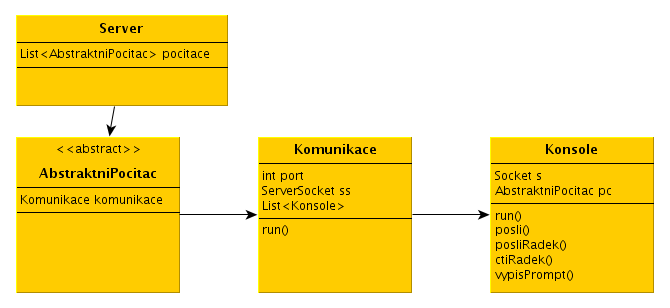
\includegraphics[width=14cm]{obrazky/komunikacni_vrstva}
\caption{Komunikační vrstva}
\label{obr_komunikacni_vrstva}
\end{center}
\end{figure}

Hlavní třídou komunikační vrstvy je třída \verb|Komunikace|. Ta se stará o veškerou komunikaci virtuálního počítače s uživatelem. Je potomkem třídy \verb|Thread|. Běží ve vlastním vlákně, které se startuje v jejím konstruktoru, a poslouchá na portu, který jí byl zadán. Pro každé nové příchozí spojení vytvoří instanci třídy \verb|Konsole|, která spojení obslouží, aby \verb|Komunikace| mohla dále poslouchat na portu a zpracovávat další spojení. Třída \verb|Konsole| je také potomkem třídy Thread. Obsluhuje jedno telnetové připojení. Drží si instanci třídy \verb|ParserPrikazu| z balíčku \verb|Prikazy| (o něm v následující kapitole). Přijímá textová data od uživatele až po enter (sekvence \verb|\r\n|), tedy vlastně načítá data po řádcích. Každý řádek, který uživatel pošle, předá parseru na zpracování a pak sama pošle uživateli prompt. Parseru poskytuje metody pro posílání textových dat uživateli. Pro uživatele tak komunikace s touto konsolí vypadá stejně jako práce s příkazovou řádkou na skutečném počítači.


\subsection{Aplikační vrstva - virtuální síť}

Před tím, než začnu popisovat implementaci jednotlivých komponent aplikační vrstvy, sluší se, popsat ji zhruba jako celek. Virtuální síť se skládá z virtuálních počítačů, což jsou objekty potomků abstraktní třídy \verb|AbstraktniPocitac|. Ty si mezi sebou voláním svých metod předávají pakety, což jsou objekty třídy \verb|Paket|. Virtuální počítače mají síťová rozhraní, což jsou objekty třídy \verb|SitoveRozhrani|. Jejich pomocí jsou počítače mezi sebou propojeny (více o infrastruktuře v \ref{infrastruktura_site})

% uml virtualni sit
\begin{figure}[h]
\begin{center}
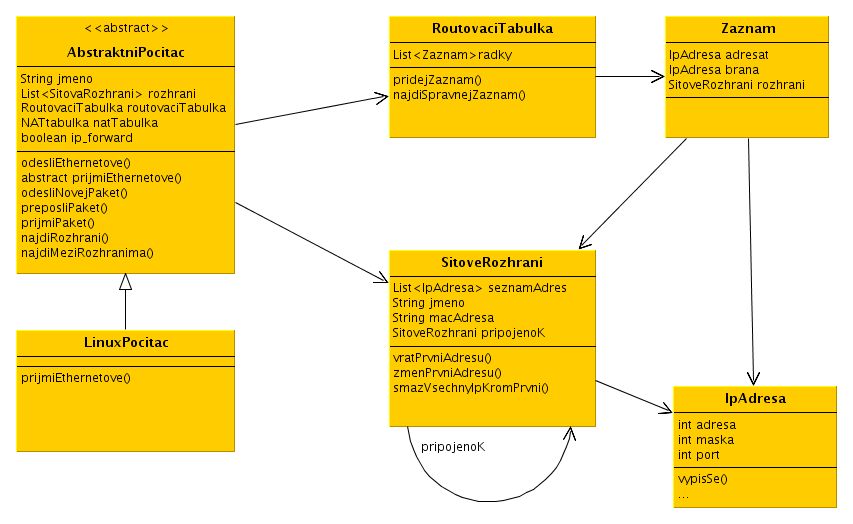
\includegraphics[width=14cm]{obrazky/virtualni_sit}
\caption{Architektura aplikační vrstvy - virtuální síť}
\label{obr_virtualni_sit}
\end{center}
\end{figure}




%----------------------------------

\section{IP adresa}

Třída \verb|IpAdresa| je sice jen jednou z mnoha tříd, vzhledem k jejímu významu ji ale v následujících odstavcích popíšu podrobněji.


\subsection{Analýza}

Protože simulátor se zabývá především simulací síťové vrstvy ISO/OSI modelu, je síťová adresa počítače, tzv. IP adresa velmi často používanou datovou strukturou, pro kterou se vyplatí mít speciální třídu. Ta se v v aplikaci jmenuje \verb|IpAdresa| a patří do balíčku \verb|datoveStruktury|. Je používána jako parametr síťového rozhraní, jako prefix v routovací tabulce, jako zdrojová a cílová adresa v paketech. Při bližším pohledu je zřejmé, že kontext jejího použití se v těchto případech částečně liší. Například pro posílání paketů je nutné, aby paket obsahoval zdrojovou a cílovou adresu i s portem. Port by samozřejmě nemusel být součástí adresy, to se ale ukázalo jako jednoduší a pro posílání paketů přehlednější možnost. Pro IP adresu jako parametr rozhraní je naopak port zcela nesmyslný parametr, nutně ale potřebuje parametr pro síťovou masku, která je naproti tomu nesmyslná pro posílání paketů. Paket posílám na IP adresu, ne na adresu s maskou.


\subsection{Vnitřní reprezentace}

Přes tyto rozdíly jsem se rozhodl vytvořit pro IP adresu jednu třídu, která má parametry \verb|adresa|, \verb|maska| a \verb|port|, přičemž pro danou situaci nepotřebné parametry prostě ignoruji. Protože Java neobsahuje žádný 32-bitový bezeznaménkový datový typ, jsou parametry adresa a maska vnitřně reprezentovány 32-bitovým integerem, který ale obsahuje bity skutečné adresy, jeho číselná hodnota není důležitá. Operace s nimi se provádí především pomocí bitových operátorů. Parametr port je normální integer.


\subsection{Veřejné metody}

\verb|IpAdresa| má konstruktory, aby ji bylo možné vytvořit ze \verb|Stringu|, s maskou zadanou jako \verb|String|, \verb|Integer| nebo v jednou řetězci s adresou. Adresu je možné převést na String nebo porovnat s jinou adresou mnoha různými způsoby, například jen podle adresy, adresy s portem, adresy s maskou nebo čísla sítě. \verb|IpAdresa| umí vrátit své číslo sítě nebo broadcast jako jinou \verb|IpAdresu|. O těchto metodách se zde nerozepisuji podrobně, v kódu jsou dobře okomentované.



%----------------------------------

\section{Virtuální počítač}

Virtuální počítač je základním stavebním prvkem naší aplikace. Pracuje na obou jejích vrstvách. Na vrstvě komunikační přijímá a zpracovává příchozí spojení, na aplikační vrstvě, tj. na vrstvě virtuální sítě přijímá, posílá a přeposílá pakety. Posíláním paketů se zabývám až v posledním odstavci této kapitoly, zde proberu komunikační vrstvu počítače a jeho rozhraní.

Protože linuxový a ciscový počítač, který dělal kolega, mají mnoho společného, vytvořil jsem abstraktní třídu \verb|AbstraktniPocitac|, který je předkem počítačů obou typů. Třída \verb|LinuxPocitac| má ale jen jednu metodu, která se týká posílání paketů, proto se jí zatím nezabývám.

Všechny virtuální počítače jsou vytvářeny v rámci inicializace aplikace dle konfiguračního souboru na začátku jejího běhu, za chodu aplikace není již možné další počítač přidat nebo nějaký odebrat. Pro komunikaci s uživatelem má každý počítač vlastní objekt třídy \verb|Komunikace|. Počítač si drží seznam svých síťových rozhraní, svoji routovací tabulku a natovací tabulku. Má jediný konstruktor, kde je mu zadáno jméno (pro přehlednost) a port, na kterém má být dostupný pro uživatele.


\subsection{Síťové rozhraní}

%v tomhle odstavci by chtěla dodělat ta footnote
Z hlediska infrastruktury sítě jsou základními prvky počítače jeho síťová rozhraní. Ty si počítač drží v seznamu. Jsou vytvořeny při parsovaní konfiguračního souboru a během běhu aplikace je nelze nijak měnit, přidávat nebo mazat. Třída \verb|SitoveRozhrani| má svoje jméno a fysickou (mac) adresu. Protože v naší aplikaci není implementován ARP\footnote{Address Resolution Protocol se v počítačových sítích s IP protokolem používá k získání ethernetové MAC adresy sousedního stroje z jeho IP adresy. Používá se v situaci, kdy je třeba odeslat IP datagram na adresu ležící ve stejné podsíti jako odesílatel. Data se tedy mají poslat přímo adresátovi, u něhož však odesilatel zná pouze IP adresu. Pro odeslání prostřednictvím např. Ethernetu ale potřebuje znát cílovou ethernetovou adresu.\cite{wiki:arp}} protokol, mac adresa nemá jiný význam, než že je vypisována příkazy jako např. \verb|ifconfig|.

Skutečné síťové rozhraní může mít více adres. Tato možnost však není v předmětu PSI využívána, proto jsem ji neimplementoval. Znamenalo by to totiž poměrně velké problémy v posílání paketů. Musel bych složitě zjišťovat, kdy se paket odešle s jakou síťovou adresou, pokud je jich na daném rozhraní více. Pro potřeby statického překladu adres (NAT) především na ciscovém routeru je ale nutné mít na rozhraní více adres\footnote{Více o překladu adres v bakalářské práci mého kolegy Stanislava Řeháka}. Proto má třída \verb|SitoveRozhrani| seznam IP adres, ale jeho první adresa je privilegovaná. Každý paket, který je přes dané rozhraní posílán, má jako odchozí adresu první adresu tohoto rozhraní. První adresa je vždy nastavená, není-li nakonfigurována, je nastavena na \verb|null|. Tuto jedinou adresu lze nastavovat a vypisovat. Ostatní adresy jsou přidávány jen pro potřeby statického natování. Pokud rozhraní nemá nastavenou žádnou adresu, je první (privilegovaná) adresa \verb|null|.



%----------------------------------

\section{Infrastruktura virtuální sítě}\label{infrastruktura_site}

Poté, co jsem popsal implementaci virtuálního počítače, můžu popsat vnitřní reprezentaci infrastruktury virtuální sítě. Ta vychází z toho, že v simulátoru neuvažuji směrovače na linkové vrstvě ISO/OSI modelu (switche). To totiž znamená, že jedno síťové rozhraní počítače může být připojeno nejvýše k jednomu jinému síťovému rozhraní nějakého počítače. Infrastruktura takové sítě je tak jednoznačně určena dvojicemi síťových rozhraní, které jsou mezi sebou propojeny kabelem. Třída \verb|SitoveRozhrani| má proto parametr \verb|pripojenoK|, který obsahuje odkaz na jiné síťové rozhraní, ke kterému je připojeno. Není-li rozhraní připojeno, je tento parametr nastaven na \verb|null|. Tato infrastruktura je samozřejmě načítána z konfiguračního souboru. Při vytváření infrastruktury aplikace ohlídá, aby rozhraní byla spojena obousměrně a správně. To jest, je-li rozhraní \verb|A| připojeno k rozhraní \verb|B|, musí být také rozhraní \verb|B| připojeno k rozhraní \verb|A|.



%----------------------------------

\section{Routovací tabulka}

% OSNOVA
% - co to je, struktura týhle části
% - použití pro cisco
% Analysa
% 	Struktura tabulky
% 	Adresát - vysvětlit, jak to funguje
% 	Příznaky
% 	Přidávání záznamů a jejich řazení
% 	Mazání záznamů
% 	Použití při směrování
% Implementace
% 	Vnitřní reprezentace (struktura)
% 	Přidávání, mazaní a řazení záznamů - jednotlivý metody, metoda pro parser konfiguráku
% 	Použití při směrování - metody

Počítače směrují pakety podle tzv. routovací, neboli směrovací, tabulky. \uv{Routovací tabulka je datový soubor uložený v RAM paměti, který je používán k uchovávání informací ohledně přímo připojených i vzdáleně připojených sítí. Její obsah napovídá routeru, kterým rozhraním je možno nejoptimálněji dosáhnout cílové sítě.}\cite{owebu:routovaci_tabulka}. V této části se zabývám nejprve analýzou routovací tabulky na skutečném linuxu a potom popisuji její implementaci v simulátoru.

Třída \verb|RoutovaciTabulka| měla být původně stejně použitelná pro linux i pro cisco. Až po tom, co jsem jí implementoval, kolega zjistil, že pro potřeby cisca není tato třída bez úprav použitelná. Proto implementoval třídu \verb|CiscoWrapper|, která obaluje třídu \verb|RoutovaciTabulka| a dodává jí funkce potřebné pro cisco. To však není obsahem mojí práce.


\subsection{Analýza routovací tabulky na skutečném počítači}

\subsubsection{Struktura tabulky}

V řádcích routovací tabulky jsou záznamy pro jednotlivé sítě. Každý záznam má tyto parametry:
\begin{itemize}
\item adresát - IP adresa s maskou, pro kterou je tento záznam platný
\item brána - IP adresa počítače, na který se má paket poslat. Tento sloupec nemusí být vždy vyplněn.
\item příznaky - O těch více píšu v samostatné části.
\item metrika - Jedno z kriterií priority.
\item rozhraní - Rozhraní, přes které se paket posílá.
\end{itemize}
Parametr metrika není pro výukové účely potřeba, proto se jím již dále nezabývám.

Pro lepší představu zde vkládám routovací tabulku tak, jak je vypsána příkazem\linebreak \verb|route -n|:
\begin{verbatim}
Adresát         Brána           Maska           Přízn Metrik Rozhraní
147.32.125.128  0.0.0.0         255.255.255.128 U     1      eth0
169.254.0.0     0.0.0.0         255.255.0.0     U     1000   eth0
0.0.0.0         147.32.125.129  0.0.0.0         UG    0      eth0
\end{verbatim}

\subsubsection{Adresát}

V hořejším výpisu tabulky pomocí příkazu \verb|route| se adresáta týkají 2 sloupce, sloupec Adresát a sloupec Maska, ve kterém jsou vypsány masky k IP adresám uvedeným ve sloupci Adresát. Tyto IP adresy s maskami jsou vždy číslem sítě a reprezentují všechny adresy, které do této sítě patří. Tak například adresát 0.0.0.0/0 reprezentuje úplně všechny IP adresy, adresát 147.32.125.128/25 reprezentuje adresy v rozmezí 147.32.125.128 až 147.32.125.255, adresát 1.1.1.1/32 reprezentuje jedinou adresu 1.1.1.1 a adresát 192.168.1.0/24 reprezentuje všechny adresy, které začínají byty 192.168.1.x. Adresáta 147.32.125.128/24 nelze zadat, protože číslo této sítě je 147.32.125.0/24.

\subsubsection{Příznaky}\label{routTabulka-priznaky}

Záznam routovací tabulky má několik příznaků. Má vždy minimálně jeden příznak, může mít ale všechny 3 příznaky najednou. Zde je jejich popis:
\begin{itemize}
\item Příznak \verb|U| znamená, že záznam obsahuje rozhraní. Protože záznam bez vyplněného rozhraní není možné zadat, má tento příznak každý záznam.
\item Záznam má příznak \verb|G|, jestliže je vyplněn sloupec brána.
\item Příznak H znamená, že adresátem daného záznamu je jeden počítač, tzn. adresát má masku 255.255.255.255.
\end{itemize}
Příznak \verb|H| jen informuje, že adresát není sítí, ale jediným počítačem, není tedy nijak důležitý. Podle příznaků existují 2 typy záznamů, záznamy s příznakem \verb|U| a záznamy s příznakem \verb|UG|. Tyto typy se liší jak při přidávání nových záznamů do routovací tabulky, tak při posílání paketu podle tohoto záznamu. Posílá-li počítač paket podle záznamu U, není z tohoto záznamu zřejmé, jakému sousednímu počítači (na linkové vrstvě) se má paket poslat. Počítač se tedy pokusí poslat paket přímo na cílovou IP adresu uvedenou v paketu. Posílá-li se paket podle záznamu UG, posílá se na adresu brány uvedenou v záznamu. Více se této problematice věnuji v kapitole o posílání paketů.

\subsubsection{Přidávání záznamů a jejich řazení}

Routovací tabulka nesmí obsahovat 2 stejné záznamy. Za stejné záznamy se považují záznamy, které mají stejného adresáta včetně masky, stejné rozhraní a stejnou bránu.

Záznam typu \verb|U| lze přidat vždycky. Záznam typu \verb|UG| lze přidat jen pod podmínkou, že jeho brána je v okamžiku přidání dosažitelná záznamem typu \verb|U|. Tím je možné dosáhnout zajímavého chování: Když do routovací tabulky přidám defaultní routu \footnote{Defaultní routa je záznam platný pro celý internet, jeho adresátem je 0.0.0.0/0} záznamu typu U, můžu pak přidat routu na jakoukoliv síť v internetu se záznamem UG. Když potom smažu původní defaultní routu, můžu posílat pakety pouze na tu síť s příznakem \verb|UG| a na počítač v mé síti paket neodešlu. Zde uvádím příklad:
\begin{verbatim}
root: /home/neiss# route add default eth0
root: /home/neiss# route add -net 89.190.94.0/24 gw 89.190.94.1
root: /home/neiss# route del default
root: /home/neiss# route
Směrovací tabulka v jádru pro IP
Adresát         Brána           Maska           Přízn Metrik Rozhraní
89.190.94.0     89.190.94.1     255.255.255.0   UG    0      eth0
\end{verbatim}
Toto je ping na nějakou adresu kdesi v internetu:
\begin{verbatim}
root: /home/neiss# ping -c1 89.190.94.58
PING 89.190.94.58 (89.190.94.58) 56(84) bytes of data.
64 bytes from 89.190.94.58: icmp_seq=1 ttl=53 time=14.1 ms

--- 89.190.94.58 ping statistics ---
1 packets transmitted, 1 received, 0% packet loss, time 0ms
rtt min/avg/max/mdev = 14.141/14.141/14.141/0.000 ms
\end{verbatim}
Toto je ping na mojí bránu, přes kterou do internetu šel i minulý paket:
\begin{verbatim}
root: /home/neiss# ping -c1 147.32.125.129
connect: Network is unreachable
\end{verbatim}
Tento pokus funguje ale jen tehdy, pokud moje brána, v tomto případě 147.32.125.129 je cisco (viz část o posílání paketů).

Záznamy se v tabulce řadí podle masky adresáta. Nahoře jsou záznamy s nejdelší maskou, tzn. záznamy nejkonkrétnější. Pokud vkládám více záznamů se stejnou maskou, chová se routovací tabulka naprosto nepředvídatelně, což je vidět na následujícím příkladě:
\begin{small}
\begin{verbatim}
node-4:/home/dsn# route add -net 1.1.8.0/25 dev eth0
node-4:/home/dsn# route add -net 1.1.9.0/25 dev eth0
node-4:/home/dsn# route add -net 1.1.10.0/25 dev eth0
node-4:/home/dsn# route add -net 1.1.11.0/25 dev eth0
node-4:/home/dsn# route add -net 1.1.12.0/25 dev eth0
node-4:/home/dsn# route add -net 1.1.13.0/25 dev eth0
node-4:/home/dsn# route add -net 1.1.14.0/25 dev eth0
node-4:/home/dsn# route add -net 1.1.15.0/25 dev eth0
node-4:/home/dsn# route
Kernel IP routing table
Destination     Gateway         Genmask         Flags Metric  Iface
1.1.10.0        *               255.255.255.128 U     0       eth0
1.1.11.0        *               255.255.255.128 U     0       eth0
1.1.8.0         *               255.255.255.128 U     0       eth0
1.1.9.0         *               255.255.255.128 U     0       eth0
1.1.14.0        *               255.255.255.128 U     0       eth0
1.1.15.0        *               255.255.255.128 U     0       eth0
1.1.12.0        *               255.255.255.128 U     0       eth0
1.1.13.0        *               255.255.255.128 U     0       eth0
\end{verbatim}
\end{small}
Podle jakého algoritmu jsou nové záznamy zařazovány je mi opravdu záhadou.

\subsubsection{Mazání záznamů}

Smazat je možno jakýkoliv záznam tabulky. Pro mazání záznamů je potřeba zadat správně minimálně adresáta záznamu. Pokud pak existuje více záznamů se zadanými parametry, smaže se první z nich. Smazání jakéhokoliv záznamu nijak neovlivní ostatní záznamy.

\subsubsection{Použití pro směrování}\label{routTabulka_pouzitiPriSmerovani}

Ke směrování paketu se použije první záznam odpovídající cílové adrese. To znamená, že bude-li v routovací tabulce dané adrese odpovídat více záznamů, použije se ten nejvíce nahoře. Protože záznamy jsou řazeny podle délky síťové masky, je vrácený záznam ten nejkonkrétnější.


\subsection{Implementace routovací tabulky v simulátoru}

Routovací tabulka je implementována třídou \verb|RoutovaciTabulka|, jejíž odkaz si drží\linebreak \verb|AbstraktniPocitac| a podle ní směruje pakety.

\subsubsection{Vnitřní reprezentace}

Tabulka je vnitřně reprezentována seznamem objektů typu \verb|Zaznam|, který reprezentuje jeden záznam, tj. řádek tabulky. Záznam routovací tabulky má v simulátoru jen tyto parametry: adresát, brána a rozhraní, které fungují tak, jak bylo popsáno v odstavci o analýze. Parametry adresát a brána jsou typu \verb|IpAdresa|, parametr rozhraní je typu \verb|SitoveRozhrani|. Parametr záznamy není vůbec potřeba. Příznak \verb|U| musí mít záznam vždy, příznak \verb|H| má právě tehdy, když adresát má masku 255.255.255.255, a příznak \verb|U| má záznam právě tehdy, když má vyplněnou položku brána, proto ani ten není potřeba.

\subsubsection{Přidávání, mazání a řazení záznamů}

Záznamy jsou přidávány pomocí 2 metod se stejným názvem \verb|pridejZaznam|, ale jinými parametry. Jedna přidává záznam typu \verb|U|, druhá, která má navíc parametr brána, záznam typu \verb|UG|. U obou se kontroluje, jestli tabulka již stejný záznam neobsahuje, u té druhé se navíc kontroluje dosažitelnost brány, jak bylo popsáno v analýze.

Záznamy se samozřejmě řadí podle masky jako v reálné tabulce, záznamy se stejnou maskou se ale vloží vždy nad původní záznam. Tak jsou novější záznamy vždy nahoře. Zmatečné řazení reálné tabulky jsem samozřejmě neimplementoval.

Pro mazání má \verb|RoutovaciTabulka| metodu \verb|SmazZaznam|, funguje stejně jako na reálném počítači.

Navíc obsahuje \verb|RoutovaciTabulka| ještě metodu \verb|pridejZaznamBezKontrol|, která je využívána při vytváření počítače z konfiguračního souboru, jinde se nepoužívá.

\subsubsection{Použití při směrování}

K samotnému směrování slouží metoda \verb|najdiSpravnyZaznam|, která vrací celý řádek routovací tabulky. Funguje stejně jako na reálném počítači.



%----------------------------------

\section{Posílání paketů}

% 	Osnova sekce:
% 	- popsat, k čemu se u nás pakety posílaj
% 	- popsat strukturu týhle části - DODĚLAT !!!
% 	Referenční model ISO/OSI
% 		- popsat vrstvy skutečný sítě, který se nás týkaj, zabalování rámců, atd
% 		Datové bloky
% 	implementace našeho paketu
% 	Chování reálného počítače při posílání paketů
% 		Trensportní vrstva - icmp
% 		Síťová vrstava - IP
% 			ip_forward
% 			Směrování
% 			ttl
% 			Next hop
% 		Linková vrstva - ethernet
% 		Zajímavosti - DODĚLAT!!!
% 	popsat implementaci
% 		- rozdělení do vrstev
% 		jednotlivý metody

Posílání paketů v naší aplikaci slouží k tomu, aby uživatel pomocí příkazů \verb|ping| a \verb|traceroute| mohl ověřit, zda síť správně nakonfiguroval. Bez této části by naší aplikaci nebylo možné nazvat síťovým simulátorem.


\subsection{Teoretický rozbor referenčního modelu ISO/OSI}

\uv{Referenční model ISO/OSI vypracovala organizace ISO jako hlavní část snahy o standardizaci počítačových sítí.}\cite{wiki:referencni_model}. Dle tohoto modelu probíhá síťová komunikace v sedmi vrstvách, z níž každá poskytuje přesně definované funkce a komunikuje jen s vrstvou sousední. Každá vrstva má svůj formát přenášených dat, obyčejně dělených do bloků. Pro moji aplikaci jsou důležité vrstvy 2 - 4, tzn. spojová, síťová a transportní vrstva.

\subsubsection{Spojová vrstva}

Spojová nebo linková vrstva\footnote{Více v \cite{wiki:linkova_vrstva}} \uv{poskytuje spojení mezi dvěma sousedními systémy.}\cite{wiki:referencni_model}. Tuto vrstvu zajišťuje na skutečné síti v laboratoři technologie Ethernet\cite{wiki:ethernet}, ke zjištění fysické adresy sousedního systému se používá protokol ARP\cite{wiki:arp}. Sousedními systémy se zde rozumí počítače zapojené do stejné sítě. Blok dat na linkové vrstvě se nazývá rámec. Vzhledem k tomu, že simulátor neobsahuje žádné switche, zajišťuje tato vrstva v naší aplikaci spojení mezi 2 počítači propojenými kabelem.

\subsubsection{Síťová vrstva}

Síťová vrstva \uv{se stará o směrování v síti a síťové adresování. Poskytuje spojení mezi systémy, které spolu přímo nesousedí.}\cite{wiki:referencni_model} Zajišťuje spojení mezi jakýmikoliv dvěma uzly sítě. Obyčejně je realizována protokolem IP\footnote{Internet Protocol}. Blok dat na síťové vrstvě se nazývá paket.

\subsubsection{Transportní vrstva}

Transportní vrstva \uv{zajišťuje přenos dat mezi koncovými uzly}\cite{wiki:referencni_model}. Pro potřeby příkazů ping a traceroute je tato vrstva realisována protokolem ICMP\footnote{Internet Control Message Protocol, více v \cite{wiki:icmp}}. Blok dat se v transportní vrstvě nazývá datagram.

\subsubsection{Datové bloky}\label{datove_bloky}

Datový blok jakékoliv vrstvy se skládá z hlavičky, která obsahuje režijní informace té vrstvy a z datové části, která obsahuje samotná data, ale i hlavičky vyšších vrstev. Tak například datagram protokolu ICMP je obalen hlavičkou IP na síťové vrstvě a hlavičkou protokolu Ethernet na spojové vrstvě.


\subsection{Implementace třídy Paket}
Pro můj síťový simulátor by bylo nesmyslné implementovat posílání paketů včetně jejich zabalování do datových bloků různých vrstev, tak jak je to popsáno v předchozím odstavci \ref{datove_bloky}. Proto jsem vytvořil třídu \verb|Paket|, která obsahuje všechny potřebné informace z datových bloků všech tří vrstev. \verb|Paket| má parametry síťové vrstvy jako zdrojovou a cílovou adresu \verb|ttl| a parametry transportní vrstvy jako typ a kód protokolu ICMP. Pro snadnější implementaci příkazu ping má parametr \verb|cas|, kam se ukládá náhodně generovaný čas běhu paketu, který vypisuje příkaz ping. Protože na jednom virtuálním počítači může běžet více příkazů \verb|ping| najednou, nese paket i odkaz na příkaz, který ho poslal, aby ho tento příkaz mohl také po jeho návratu zpracovat.

Typy a kódy ICMP paketů jsou označeny stejně jako ve skutečnosti:
\begin{itemize}
\item typ 0 - ozvěna (icmp reply) - odpověď na požadavek icmp request
\item typ 3 - vyslaný paket nemohl být doručen
\item typ 8 - žádost o ozvěnu (icmp request)
\begin{itemize}
\item kód 0 - network unreachable (nedosažitelná síť)
\item kód 1 - host unreachable (nedosažitelná adresa)
\end{itemize}
\item typ 11 - \verb|ttl| vypršelo
\end{itemize}


\subsection{Chování reálného počítače při posílání paketů}

\subsubsection{Transportní vrstva - protokol ICMP}

V souboru \verb|/proc/sys/net/ipv4/icmp_echo_ignore_all| je nastaveno, jestli počítač odpovídá na dotazy icmp reply. Pokud je v tomto souboru \verb|0|, počítač na dotazy odpovídá. Toto je defaultní nastavení, proto jsem v simulátoru tento problém vůbec neřešil a počítač odpovídá na icmp request vždy.

\subsubsection{Síťová vrstva - protokol IP}

\paragraph{Přeposílání paketů}
Počítač přeposílá pakety jenom tehdy, pokud je v souboru \verb|/proc/sys/net/ipv4/ip_forward| jednička, jinak ne. Toto nastavení ale již není defaultní, proto ho musím v simulátoru implementovat. Proměnná \verb|ip_forward| je parametrem virtuálního počítače a je nastavována pomocí příkazu \verb|echo|.
\paragraph{Směrování paketů}
Pakety jsou směrovány podle routovací tabulky, kde se vybere první záznam odpovídající cílové adrese paketu, jak je popsáno v \ref{routTabulka_pouzitiPriSmerovani}. Pokud v routovací tabulce nebyl nalezen žádný záznam pro cílovou adresu paketu, pošle se na jeho zdrojovou adresu paket \verb|icmp_net_unreachable|\footnote{Tj ICMP paket typu 3 kódu 0}.
\paragraph{ttl}
Každý prvek, který pracuje i na síťové vrstvě sníží procházejícím paketům hodnotu \verb|ttl|. Pokud po tomto snížení dosáhne hodnota \verb|ttl| nuly, pošle počítač na zdrojovou adresu paketu zprávu \verb|icmp_ttl_exceeded|\footnote{Tj. icmp paket typu 11}.
\paragraph{Next hop}
Předtím než síťová vrstva předá odeslání paketu linkové vrstvě, musí pro tento paket zjistit tzv. next hop, neboli sousední adresu. \uv{Next hop je sousední směrovač, na který je paket poslán nebo přeposlán z daného směrovače na své cestě k cíli.}\cite{next_hop} Tato adresa je velmi důležitá pro linkovou vrstvu, která paket posílá právě na tuto adresu. Pokud je paket směrován podle záznamu typu \verb|UG| (viz \ref{routTabulka-priznaky}), je adresa next hop uvedena ve sloupci brána routovací tabulky. Pokud je paket směrován podle záznamu typu \verb|U|, je adresa next hop cílová adresa paketu. Podle routovací tabulky
\begin{verbatim}
Adresát         Brána           Maska           Přízn Metrika  Rozhraní
147.32.125.128  0.0.0.0         255.255.255.128 U     0       eth0
0.0.0.0         147.32.125.129  0.0.0.0         UG    0       eth0
\end{verbatim}
je pro pakety směrované podle prvního záznamu next hop rovná jejich cílové adrese. Pro pakety směrované podle druhého záznamu je next hop \verb|147.32.125.129|. Záznamy typu \verb|U| jsou tak používány pro počítače v mé síti, které jsou dosažitelné přímo bez jakéhokoliv mezilehlého směrovače. Záznamy \verb|UG| jsou používány pro počítače, na které je paket posílán přes jeden nebo více směrovačů.

\subsubsection{Linková vrstva}\label{skutecna_linkova_vrstva}

Na linkové vrstvě se rámce přeposílají jen mezi sousedními počítači. Běžně ji zajišťuje protokol Ethernet. IP adresu sousedního počítače, na kterou má rámec poslat, next hop, dostane od síťové vrstvy, musí ji přeložit na fysickou (MAC\footnote{Media Access Control}) adresu, což dělá protokolem ARP. Protokol ARP vyšle ethernetový rámec na všechny okolní počítače žádost, která obsahuje zadanou IP adresu. Pokud některý z počítačů má tokovou IP adresu, původnímu počítači pošle zpátky svoji fysickou adresu a ten pak může odeslat paket. Aby počítač nemusel fysickou adresu zjišťovat při odesílání každého rámce, ukládá si v datové struktuře nazvané ARP tabulka záznamy s IP adresami, které již dříve překládal.

Pokud počítač nemůže linkovou vrstvou odeslat rámec (paket), například proto, že počítač s takovou adresou na síti neexistuje, pošle původnímu odesílateli ICMP paket\linebreak \verb|net unreachable|\footnote{Tj. ICMP paket typu 3 kódu 1}.

% ethernetový problémy na ciscu:
Počítač s operačním systémem linux odpovídá na ARP dotazy jen tehdy, když má požadovanou IP adresu nastavenou na svém rozhraní. V tom se liší od cisca, které na ARP dotaz odpoví i v případě, že adresu na svém rozhraní nemá, ale ví, kam má paket dále směrovat, tzn. má pro požadovanou adresu záznam v routovací tabulce, a naopak na ARP dotaz neodpoví v případě, že nemá v routovací tabulce záznam pro IP adresu, odkud dotaz přišel. Pro lepší pochopení přepisuji podmínku ještě v jazyce booleovských výrazů:\\
Cisco odpoví na ARP dotaz právě tehdy, když:\\
Má záznam v routovací tabulce pro počítač, který ARP dotaz posílá \verb|a zároveň| (Má nastavenou požadovanou IP adresu \verb|nebo| Má záznam v routovací tabulce pro cílovou adresu posílaného paketu)

\subsubsection{Zajímavá zjištění}

Při analýze chování linuxového počítače v síťové komunikaci jsem zjistil několik zajímavých a aspoň pro mě překvapujících faktů. Například 2 počítače v síti spolu můžou komunikovat i tehdy, mají-li nastaveny IP adresy z úplně jiných sítí. Stačí totiž, mají-li v routovací tabulce jeden na druhého záznam. Počítače z obrázku \ref{obr_divna_sit} spolu opravdu komunikují, jak je vidět na následujícím výpisu.

% divná síť
\begin{figure}[h]
\begin{center}
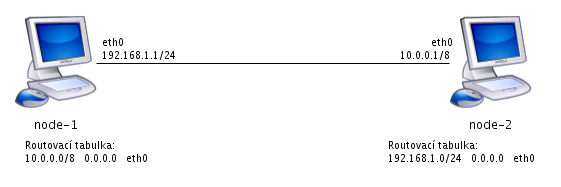
\includegraphics[width=12cm]{obrazky/divna_sit}
\caption{Funkční síť se \uv{špatnými} adresami}
\label{obr_divna_sit}
\end{center}
\end{figure}

\begin{verbatim}
node-1:/home/dsn# ifconfig eth0
eth0      Link encap:Ethernet  HWaddr 00:40:F4:B7:F0:32
          inet addr:192.168.1.1  Bcast:192.168.1.255  Mask:255.255.255.0
          inet6 addr: fe80::240:f4ff:feb7:f032/64 Scope:Link
          UP BROADCAST RUNNING MULTICAST  MTU:1500  Metric:1
          RX packets:43 errors:0 dropped:0 overruns:0 frame:0

node-1:/home/dsn# ping 10.0.0.1
PING 10.0.0.1 (10.0.0.1) 56(84) bytes of data.
64 bytes from 10.0.0.1: icmp_seq=1 ttl=64 time=0.942 ms
64 bytes from 10.0.0.1: icmp_seq=2 ttl=64 time=0.208 ms

--- 10.0.0.1 ping statistics ---
2 packets transmitted, 2 received, 0% packet loss, time 1003ms
rtt min/avg/max/mdev = 0.191/0.447/0.942/0.350 ms

\end{verbatim}


\subsection{Implementace v simulátoru}

Pakety jsou mezi počítači posílány vzájemným voláním metod, které si mezi sebou předávají objekt typu \verb|Paket|. Všechny tyto metody jsou ve třídě \verb|AbstraktniPocitac|, protože to jsou právě virtuální počítače, které si mezi sebou pakety posílají. Jen metoda \verb|prijmiEthernetove| je sice v \verb|AbstraktniPocitac| deklarována, ale implementována v jeho potomcích.


Metody virtuálního počítače pro posílání paketů jsem bylo rozumné implementovat dle vrstev. Je to přehlednější, než kdybych měl jednu metodu pro přijmutí paketu a je to dobré i vzhledem k tomu, že linux a cisco se v některých případech liší a to jen na některých vrstvách. Metody jedné vrstvy tak volají jen metody vrstvy sousední, jako na reálné síti jedna vrstva komunikuje jen s vrstvami sousedními.

\subsubsection{Linková vrstva}

ARP protokol na zjišťování fysických adres nemusel být implementován, protože v síti nejsou žádné switche a v linkové vrstvě tak není potřeba žádné směrování. Aby ale byly splněny podmínky doručení nebo nedoručení paketu uvedené v \ref{skutecna_linkova_vrstva}, byly vytvořeny metody \verb|odesliEthernetove| a \verb|prijmiEthernetove|, které si mezi sebou předávají pakety tak, aby byly tyto podmínky splněny. Metoda \verb|odesliEthernetove| je volána nějakou metodou síťové vrstvy. Pokouší se odeslat paket tak, že zavolá metodu \verb|prijmiEthernetove| nějakého jiného počítače. Metoda \verb|prijmiEthernetove| na linuxu přijme paket jen tehdy, pokud souhlasí očekávaná adresa, tj. adresa next hop odesílacího počítače. Přijme tedy paket právě tehdy, když by skutečný počítač odpověděl na ARP dotaz. Pokud se metodě \verb|odesliEthernetove| nepovede paket odeslat proto, že ho metoda \verb|prijmiEthernetove| odmítla, pošle odesílateli pomocí metody \verb|posliNovejPaketOdpoved| zprávu \verb|icmp host unreachable|. Pokud metoda \verb|prijmiEthernetove| paket přijme, zavolá metodu \verb|prijmiPaket| síťové vrstvy.

\subsubsection{Síťová vrstva}

Na síťové vrstvě si pakety předávají metody \verb|odesliNovejPaket|, \verb|preposliPaket| a\linebreak \verb|prijmiPaket|. Tyto metody směrují pakety dle routovací tabulky a provádí překlad adres podle natovací tabulky. Všechny pakety přijímá metoda \verb|prijmiPaket|, která se nejdříve pokusí přeložit cílové adresy paketů. Pak rozhodne, je-li přijatý paket na tom počítači v cíli, nebo jestli se má dále přeposlat a případně zavolá metodu \verb|preposliPaket| nebo paket nějak zpracuje, například odpoví na \verb|icmp request|. Metoda \verb|preposliPaket| přeposílá pakety, když má nastaveno \verb|ip_forward|, a přeposílaným paketům snižuje ttl. Při odeslání se pokouší přeložit zdrojovou adresu paketu. Metoda \verb|odesliNovyPaket| slouží k odesílání všech nových paketů vytvořených na tom počítači.

\subsubsection{Transportní vrstva}

Do transportní vrstvy patří více metod, které slouží k posílání různých typů ICMP paketů. Například \verb|posliIcmpRequest|, \verb|posliNetUnreachable| a další. Všechny tyto metody volají metodu \verb|odesliNovyPaket| ze síťové vrstvy.
  
  
